\section{Palíndromos}

\subsection{MT Determinista de 1 cinta}

\subsubsection*{Diseño propuesto}
El algoritmo de resolución es el siguiente:

\begin{itemize}
    \item Ciclo:
    \begin{enumerate}[1.]
        \item Si no hay ninguna letra, poner un \texttt{1} (son palíndromos) y \textbf{parar}.
        \item Borrar una letra en el extremo izquierdo.
        \item Buscar la letra correspondiente en el extremo derecho.
        \item Si la letra coincide:
        \begin{enumerate}[1.]
            \item Borrarla.
            \item Volver al extremo izquierdo.
        \end{enumerate}
        \item En caso contrario:
        \begin{enumerate}[1.]
            \item Volver al extremo izquierdo, borrando todas las letras.
            \item Poner un \texttt{0} (no son palíndromos) y \textbf{parar}.
        \end{enumerate}
    \end{enumerate}
\end{itemize}

La implementación en JFLAP queda representada en la Figura \ref{fig:MT-0A}.

\begin{figure}[h]
    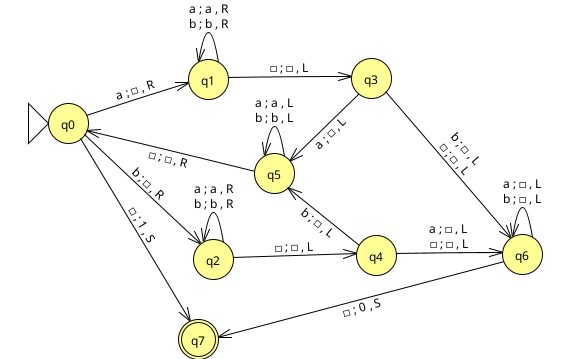
\includegraphics[width=\textwidth]{MT-0A.png}
    \caption{Implementación en JFLAP de MT-0A}
    \label{fig:MT-0A}
\end{figure}


\subsubsection*{Peor caso}
El peor caso sería cuando es un palíndromo, dado que en el momento en el que una letra no coincida, deja de buscar el resto de letras. Dentro de los palíndromos, el peor caso es cuando es un palíndromo de tamaño par, ya que tiene que hacer una comprobación extra.

\subsubsection*{Análisis empírico}

Realizamos el análisis empírico en el peor caso, tomando como $n$ el tamaño de la palabra, y midiendo el número de pasos realizados para resolver el problema\footnote{Los datos se pueden encontrar en \texttt{data/MT-0A.csv}.}:

\begin{table}[h]
    \centering
    \begin{tabular}{lcc}
        Entrada & $n$ & Pasos \\
        \hline
        $\lambda$      & 0  & 1  \\
        aa             & 2  & 6  \\
        abba           & 4  & 15 \\
        abaaba         & 6  & 28 \\
        aaabbaaa       & 8  & 45 \\
        bbaabbaabb     & 10 & 66 \\
        bbbbbaabbbbb   & 12 & 91
    \end{tabular}
\end{table}


\subsubsection*{Evaluación analítica}
Para obtener el coste computacional del algoritmo, aplicaremos Diferencias Finitas:

\begin{table}[h]
    \centering
    \begin{tabular}{|l|c|c|c|c|c|c|c|}
        \hline
        $n$ & \textbf{0} & \textbf{2} & \textbf{4} & \textbf{5} & \textbf{8} & \textbf{10} & \textbf{12} \\ \hline
        Pasos & \textbf{1} & \textbf{6} & \textbf{15} & \textbf{28} & \textbf{45} & \textbf{66} & \textbf{91} \\ \hline
        \hline
        $A(n) = T(n) - T(n-2)$ &    &  5 &  9 & 13 & 17 & 21 & 25 \\ \hline
        $B(n) = A(n) - A(n-2)$ &    &  4 &  4 &  4 &  4 &  4 &    \\ \hline
        $C(n) = B(n) - B(n-2)$ &    &    &  0 &  0 &  0 &  0 &    \\ \hline
    \end{tabular}
\end{table}

Al ser constantes las diferencias finitas segundas, y nulas las terceras, podemos aproximar $T(n)$ con un polinomio de segundo orden, es decir, $T(n) = an^2 + bn + c$.\\

Para obtener los valores de $a$, $b$, y $c$, usaremos valores de $n$ y $T(n)$ obtenidos en la evaluación empírica:

\begin{subequations}
    \begin{gather}
        n = 0,\ T(0) = 1 \rightarrow c = 1 \\
        n = 2,\ T(0) = 6 \rightarrow 4a + 2b + c = 6 \\
        n = 4,\ T(0) = 15 \rightarrow 16a + 4b + c = 6
    \end{gather}
\end{subequations}

Resolviendo, $a=\frac{1}{2}$ y $b=\frac{3}{2}$, por lo que:

\begin{equation}
    T_{0A}(n) = 2N^2 + 6N + 2
\end{equation}


\subsubsection*{Cota asintótica}

La cota asintótica queda defida como:

\begin{equation}
    O(n) = k \cdot g(n) \geq T(n)
\end{equation}

Donde $g(n)$ representa el orden de la cota superior, en este caso $g(n) = n^2$.\\

Al conocer $T_{0A}(n)$, si asumimos $n_0 = 10$, obtenemos $k \geq \frac{131}{50}$, por lo que la cota asintótica para esta máquina es:
\begin{equation}
    O_{0A}(n) = \frac{131}{50} n^2
\end{equation}


% TODO: Pintar cota asintótica y coste computacional


\subsection{MT Determinista de 2 cintas}

\subsubsection*{Diseño propuesto}
El algoritmo de resolución es el siguiente:

\begin{enumerate}
    \item Copiar los símbolos de la cinta 0 a la cinta 1.
    \item Rebobinar la cinta 1.
    \item Cotejar los símbolos de la cinta 0 y la cinta 1, avanzando ambas cintas paso a paso.
    \begin{enumerate}[1.]
        \item Si en algún punto no coinciden, rebobinar la cinta 0, limpiar la cinta 1, poner un \texttt{0} (no son palíndromos) y \textbf{parar}.
    \end{enumerate}
    \item Rebobinar la cinta 0, limpiar la cinta 1, poner un \texttt{1} (son palíndromos) y \textbf{parar}.
\end{enumerate}

La implementación en JFLAP queda representada en la Figura \ref{fig:MT-0B}.

\begin{figure}[h]
    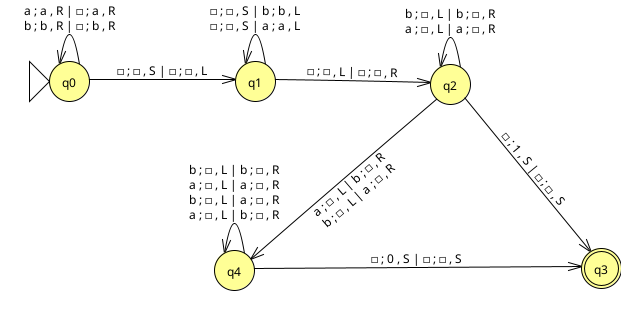
\includegraphics[width=\textwidth]{MT-0B.png}
    \caption{Implementación en JFLAP de MT-0B}
    \label{fig:MT-0B}
\end{figure}

\subsubsection*{Peor caso}
El peor caso vuelve a ser un palíndromo par, puesto que tiene que comprobar toda la cadena.

\subsubsection*{Análisis empírico}

Realizamos el análisis empírico en el peor caso, tomando como $n$ el tamaño de la palabra, y midiendo el número de pasos realizados para resolver el problema\footnote{Los datos se pueden encontrar en \texttt{data/MT-0B.csv}.}:

\begin{table}[h]
    \centering
    \begin{tabular}{lcc}
        Entrada & $n$ & Pasos \\
        \hline
        $\lambda$      & 0  & 1  \\
        aa             & 2  & 9  \\
        abba           & 4  & 15 \\
        abaaba         & 6  & 21 \\
        aaabbaaa       & 8  & 27 \\
        bbaabbaabb     & 10 & 33 \\
        bbbbbaabbbbb   & 12 & 39
    \end{tabular}
\end{table}


\subsubsection*{Evaluación analítica}
Para obtener el coste computacional del algoritmo, aplicaremos Diferencias Finitas:

\begin{table}[h]
    \centering
    \begin{tabular}{|l|c|c|c|c|c|c|c|}
        \hline
        $n$ & \textbf{0} & \textbf{2} & \textbf{4} & \textbf{5} & \textbf{8} & \textbf{10} & \textbf{12} \\ \hline
        Pasos & \textbf{1} & \textbf{6} & \textbf{15} & \textbf{28} & \textbf{45} & \textbf{66} & \textbf{91} \\ \hline
        \hline
        $A(n) = T(n) - T(n-2)$ &    &  5 &  9 & 13 & 17 & 21 & 25 \\ \hline
        $B(n) = A(n) - A(n-2)$ &    &  4 &  4 &  4 &  4 &  4 &    \\ \hline
        $C(n) = B(n) - B(n-2)$ &    &    &  0 &  0 &  0 &  0 &    \\ \hline
    \end{tabular}
\end{table}

Al ser constantes las diferencias finitas segundas, y nulas las terceras, podemos aproximar $T(n)$ con un polinomio de segundo orden, es decir, $T(n) = an^2 + bn + c$.\\

Para obtener los valores de $a$, $b$, y $c$, usaremos valores de $n$ y $T(n)$ obtenidos en la evaluación empírica:

\begin{subequations}
    \begin{gather}
        n = 0,\ T(0) = 1 \rightarrow c = 1 \\
        n = 2,\ T(0) = 6 \rightarrow 4a + 2b + c = 6 \\
        n = 4,\ T(0) = 15 \rightarrow 16a + 4b + c = 6
    \end{gather}
\end{subequations}

Resolviendo, $a=\frac{1}{2}$ y $b=\frac{3}{2}$, por lo que:

\begin{equation}
    T_{0A}(n) = 2N^2 + 6N + 2
\end{equation}


\subsubsection*{Cota asintótica}

La cota asintótica queda defida en 

\begin{equation}
    O(n) = k \cdot g(n) \geq T(n)
\end{equation}

Donde $g(n)$ representa el orden de la cota superior, en este caso $g(n) = n^2$.\\

Al conocer $T_{0A}(n)$, si asumimos $n_0 = 10$, obtenemos $k \geq \frac{131}{50}$, por lo que la cota asintótica para esta máquina es:
\begin{equation}
    O_{0A}(n) = \frac{131}{50} n^2
\end{equation}

